
\section{Metodología}

La metodología usada para la construcción del mapa de irradiación solar se la puede ver en la figura~\ref{fig:metodology}

\begin{figure}
  \centering
  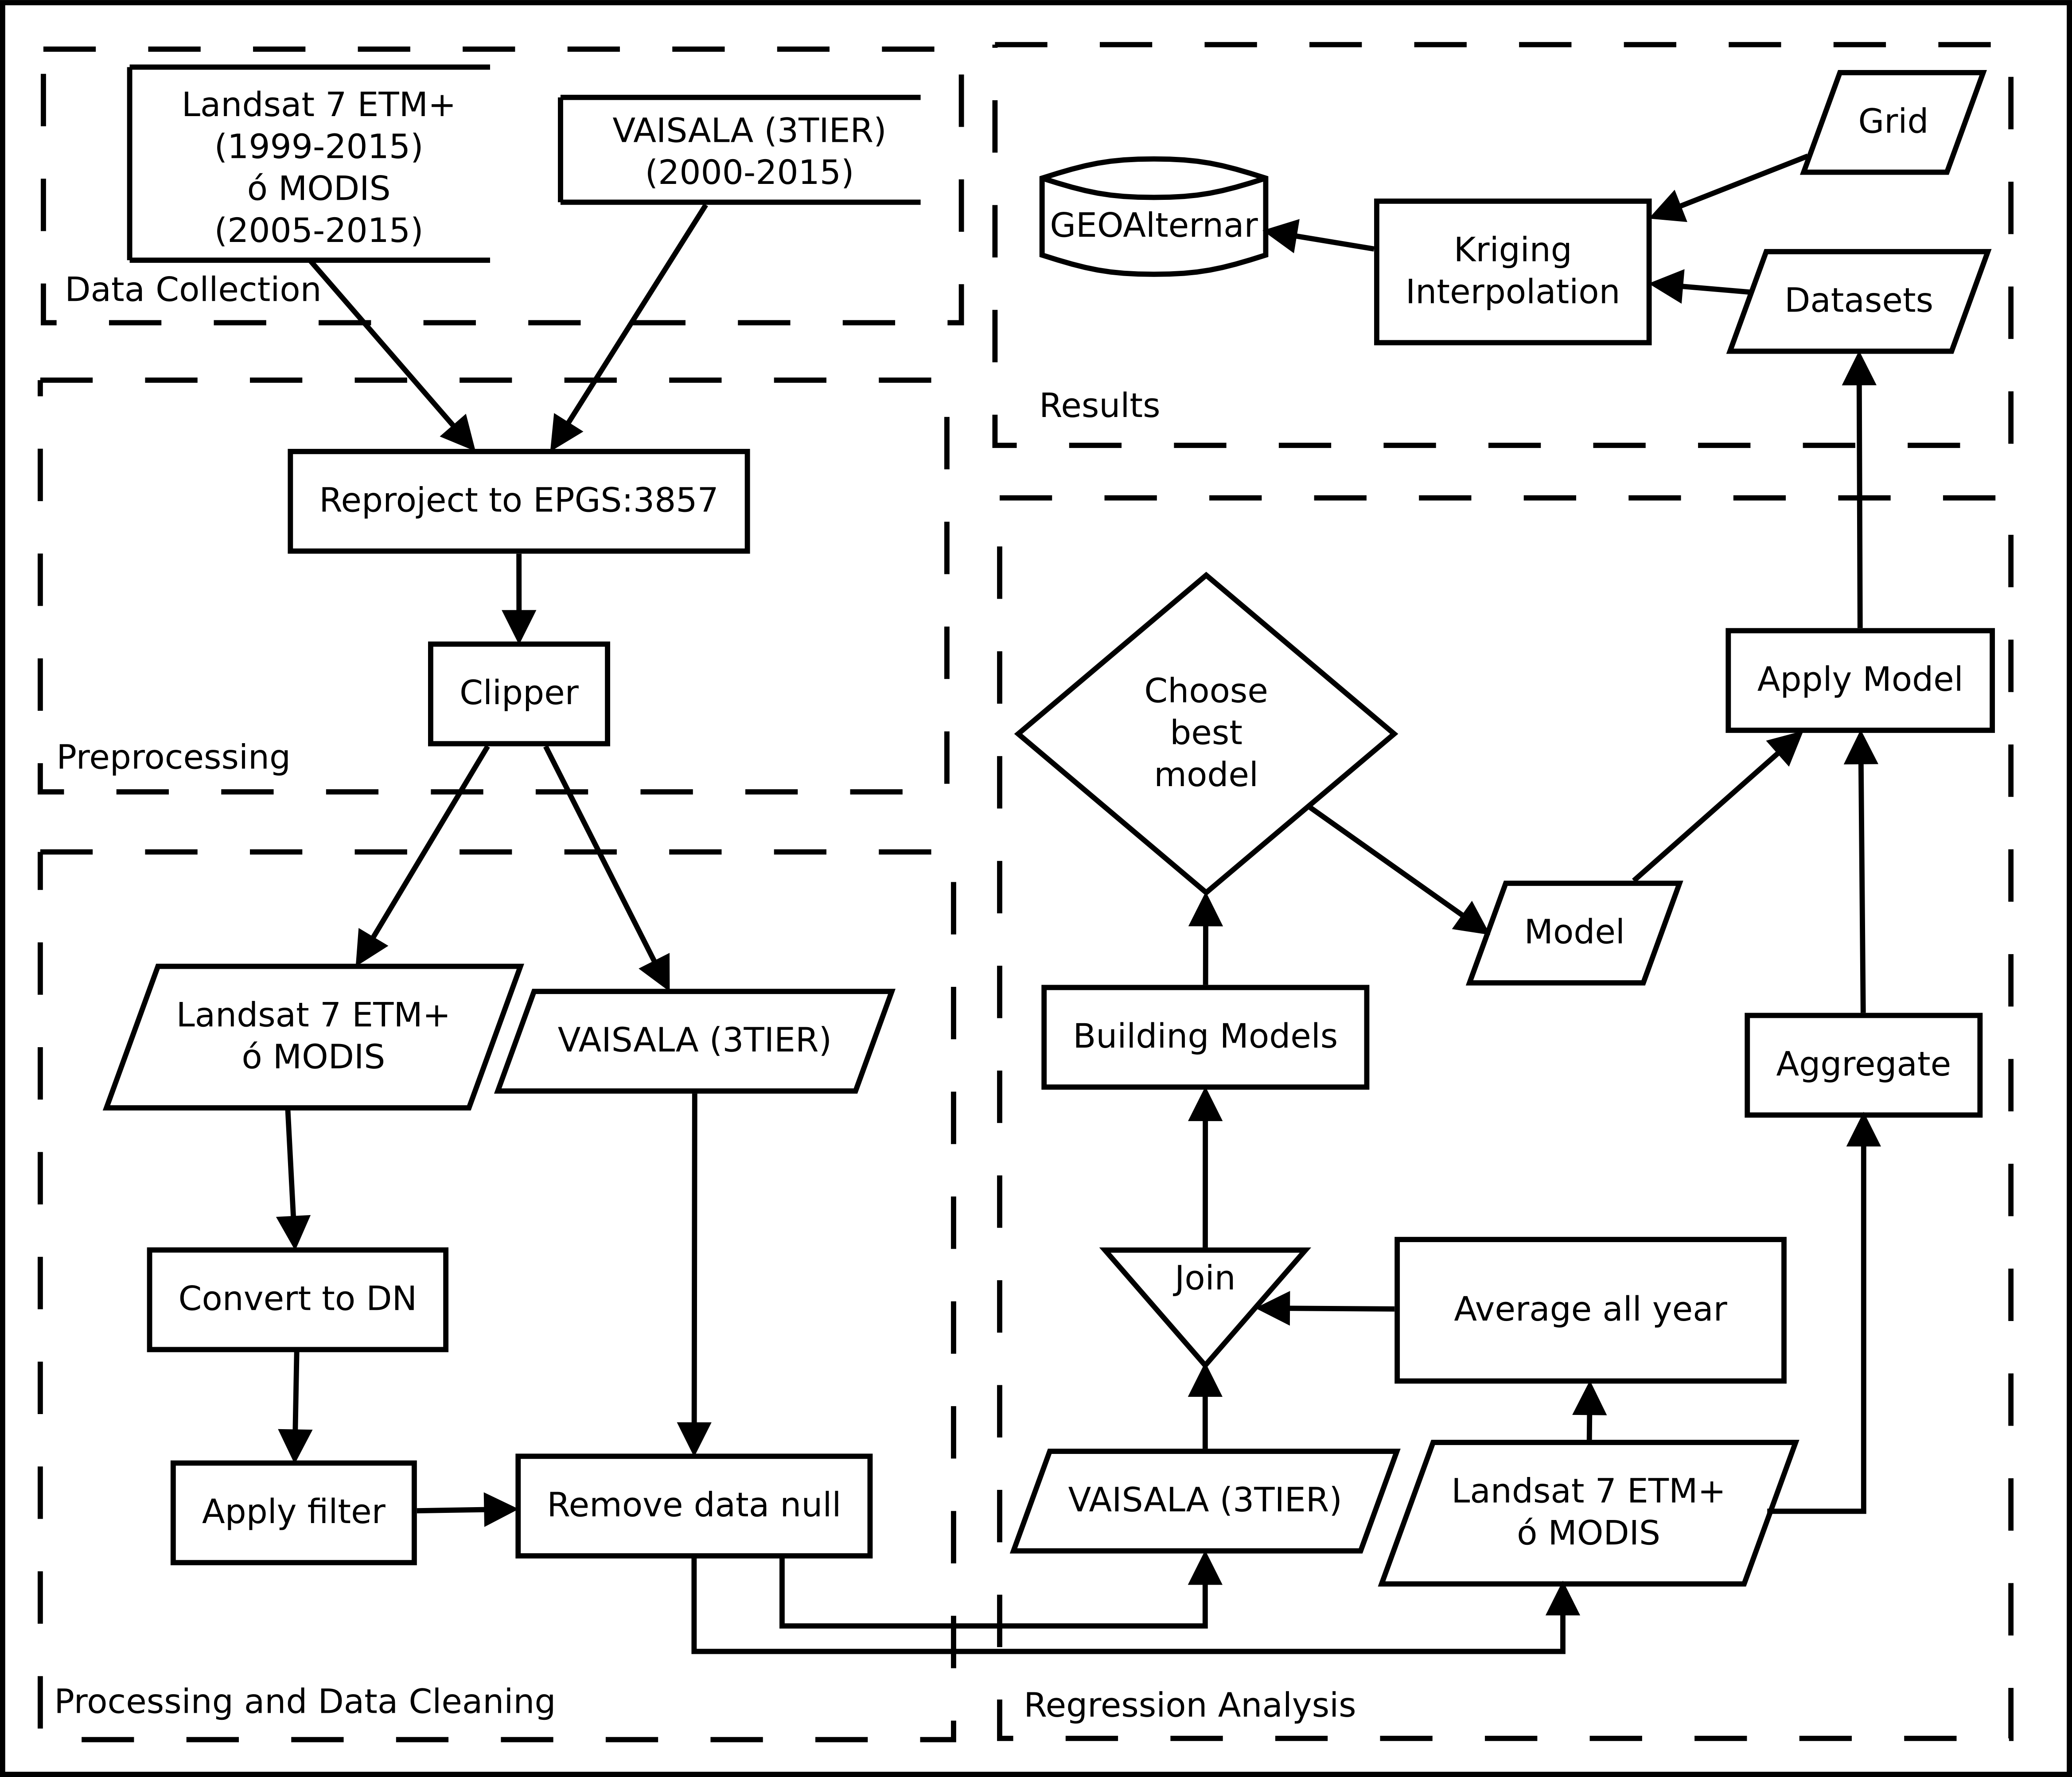
\includegraphics[width = 8cm]{metodology.png}
  \caption{Metodología}
  \label{fig:metodology}
\end{figure}

\subsection{Obtención de datos}

Se realiza el estudio de las imágenes satelitales más pertinentes para obtener la información, para la elección se tiene 
en cuenta 4 factores importantes \textit{resolución espacial}, \textit{resolución espectral}, \textit{resolución radiométrica} 
y \textit{resolución temporal} de la imágen satelital; Las imágenes de LandSat 7 son generadas cada 16 dias y permiten adquirir
datos de 8 bandas espectrales con una resolución de 15 x 15 metros por pixel para la banda 6, y 30 x 30 metros por pixel para las 7 bandas restantes, 
estas bandas tienen la capacidad de detectar diferentes indicadores para vegetación, reflectancia, temperatura, precipitación, 
nubosidad, etc. Por otra parte, las imágenes satelitales MODIS adquieren datos de 36 bandas espectrales con las cuales ofrece 
el producto MOD09GA con una resolución espacial aproximada de 500 x 500 metros en cada pixel, estos productos son generados diariamnete 
y estan diseñado para medir la reflectancia de la superficie terrestre\cite{mod09gadetails}\cite{modisweb}, MOD09GA 
presenta 7 bandas que tienen relación directa con la delimitación de territorios, tipos de vegetación, incidencia de aerosoles, 
temperatura y reflectancia la cual está relacionada con la propiedad reflectiva de la vegetación y los aerosoles; mediante la propiedad 
reflectiva de la vegetación se pretende realizar una estimación para la radiación solar que se irádia en una superficie.

Se descargaron 1362 imágenes satelitales de Landsat 7 desde
 el año 1999 hasta el año 2015, que cubren el 
departamento de Nariño, para cubrir todo el departamento fue necesario descargar las imagenes satelitales con 
los siguientes paths y rows: (009,059), (009,060), (010,058), (010,059), (011,059). 
Las imágenes satelitales de MODIS estan ubicadas en una grilla senosoidal de aproximadamente 10x10 grados 
cada sección  como lo muestra la figura~\ref{fig:gridmodis}, esta grilla cuenta 
con un índice vertical y un índice horizontal que permiten ubicar la imagen satelital en
un área determinada; el territorio colombiano se encuentra 
ubicado en la columna 10 (h10) en la fila 8 (v8) como lo muestra la figura~\ref{fig:colombiagridmodis}, estos dos indices son necesarios 
para realizar la descarga de todas las imágenes satelitales comprendidas entre el año 2005 y 2015, en estos 11 años se 
descargaron 3912 imágenes satelitales.

\begin{figure}
  \centering 
  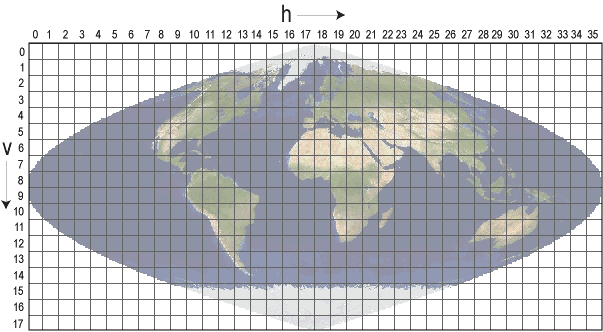
\includegraphics[width = 8cm]{MODIS_sinusoidal_grid.png}
  \caption{Grilla senosoidal de MODIS} 
  \label{fig:gridmodis}
\end{figure}

\begin{figure}
  \centering 
  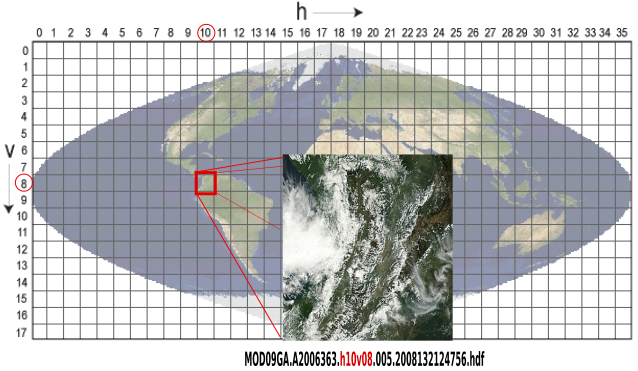
\includegraphics[width = 8cm]{mipc.png}
  \caption{Ubicación en grilla senosoidal de MODIS} 
  \label{fig:colombiagridmodis}
\end{figure}

En la obtención de datos también se utilizó el mapa de irradiancia solar proporcionado por VAISALA INC (3TIER), en el cual
se tomaron 500 muestras bien distribuidas dentro del departamento de Nariño, como lo muestra la figura~\ref{fig:3tier}.

\begin{figure}
  \centering
  \subfigure[Muestras Uniformemente distribuidas en el Departamento de Nariño]
  {\label{Muestras Uniformemente distribuidas en el Departamento de Nariño} 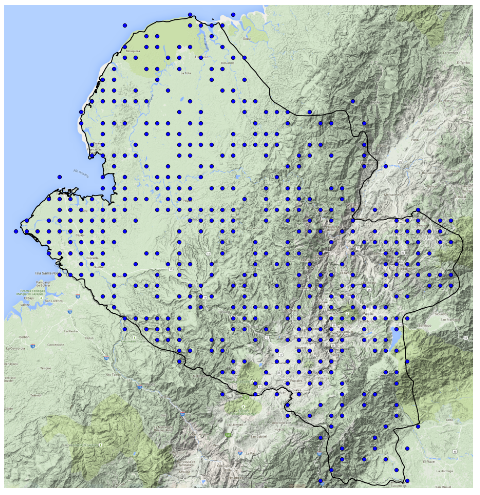
\includegraphics[width= 7cm]{m3tn.png}}
  \vfill
  \subfigure[Consulta de radiación en 3TIER]{\label{Consulta de radiación en 3TIER} 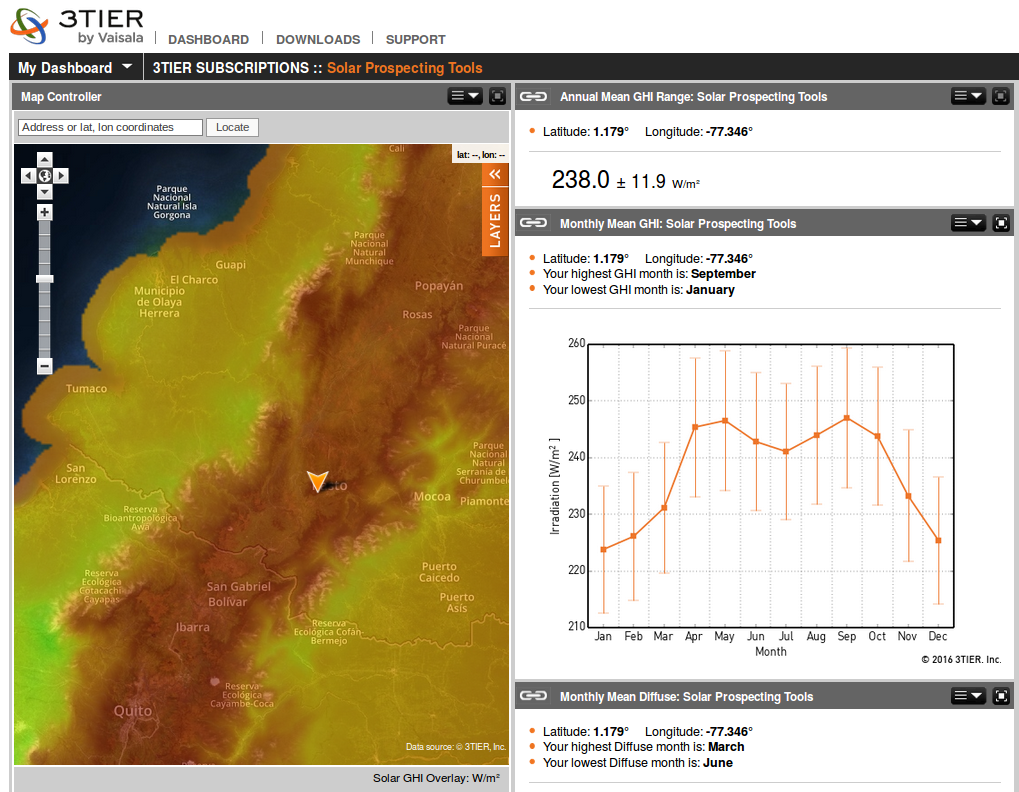
\includegraphics[width = 7cm]{3t.png}}
  \caption{Muestreo de radiación solar}
  \label{fig:3tier}
\end{figure}


\subsection{Preprocesamiento}

En la etapa de preprocesamiento para la imágenes satelitales Landsat 7, se reproyecto las imágenes obtenidas, debido a que las cinco imágenes
que cubren el departamento de Nariño, estan en distintos sistemas de coordenadas (EPSG:32618 y EPSG:32617) y se 
lo reproyecto al sitema EPSG:3857. Así como también se recorto las imágenes con el fin de unicamente tener 
el área que cubre el departamento de Nariño, como lo muestra la figura~\ref{fig:Recortar imágenes}.

\begin{figure}
  \centering
  \subfigure[Imágenes Satélitales de Nariño]{\label{Imágenes Satélitales de Nariño} 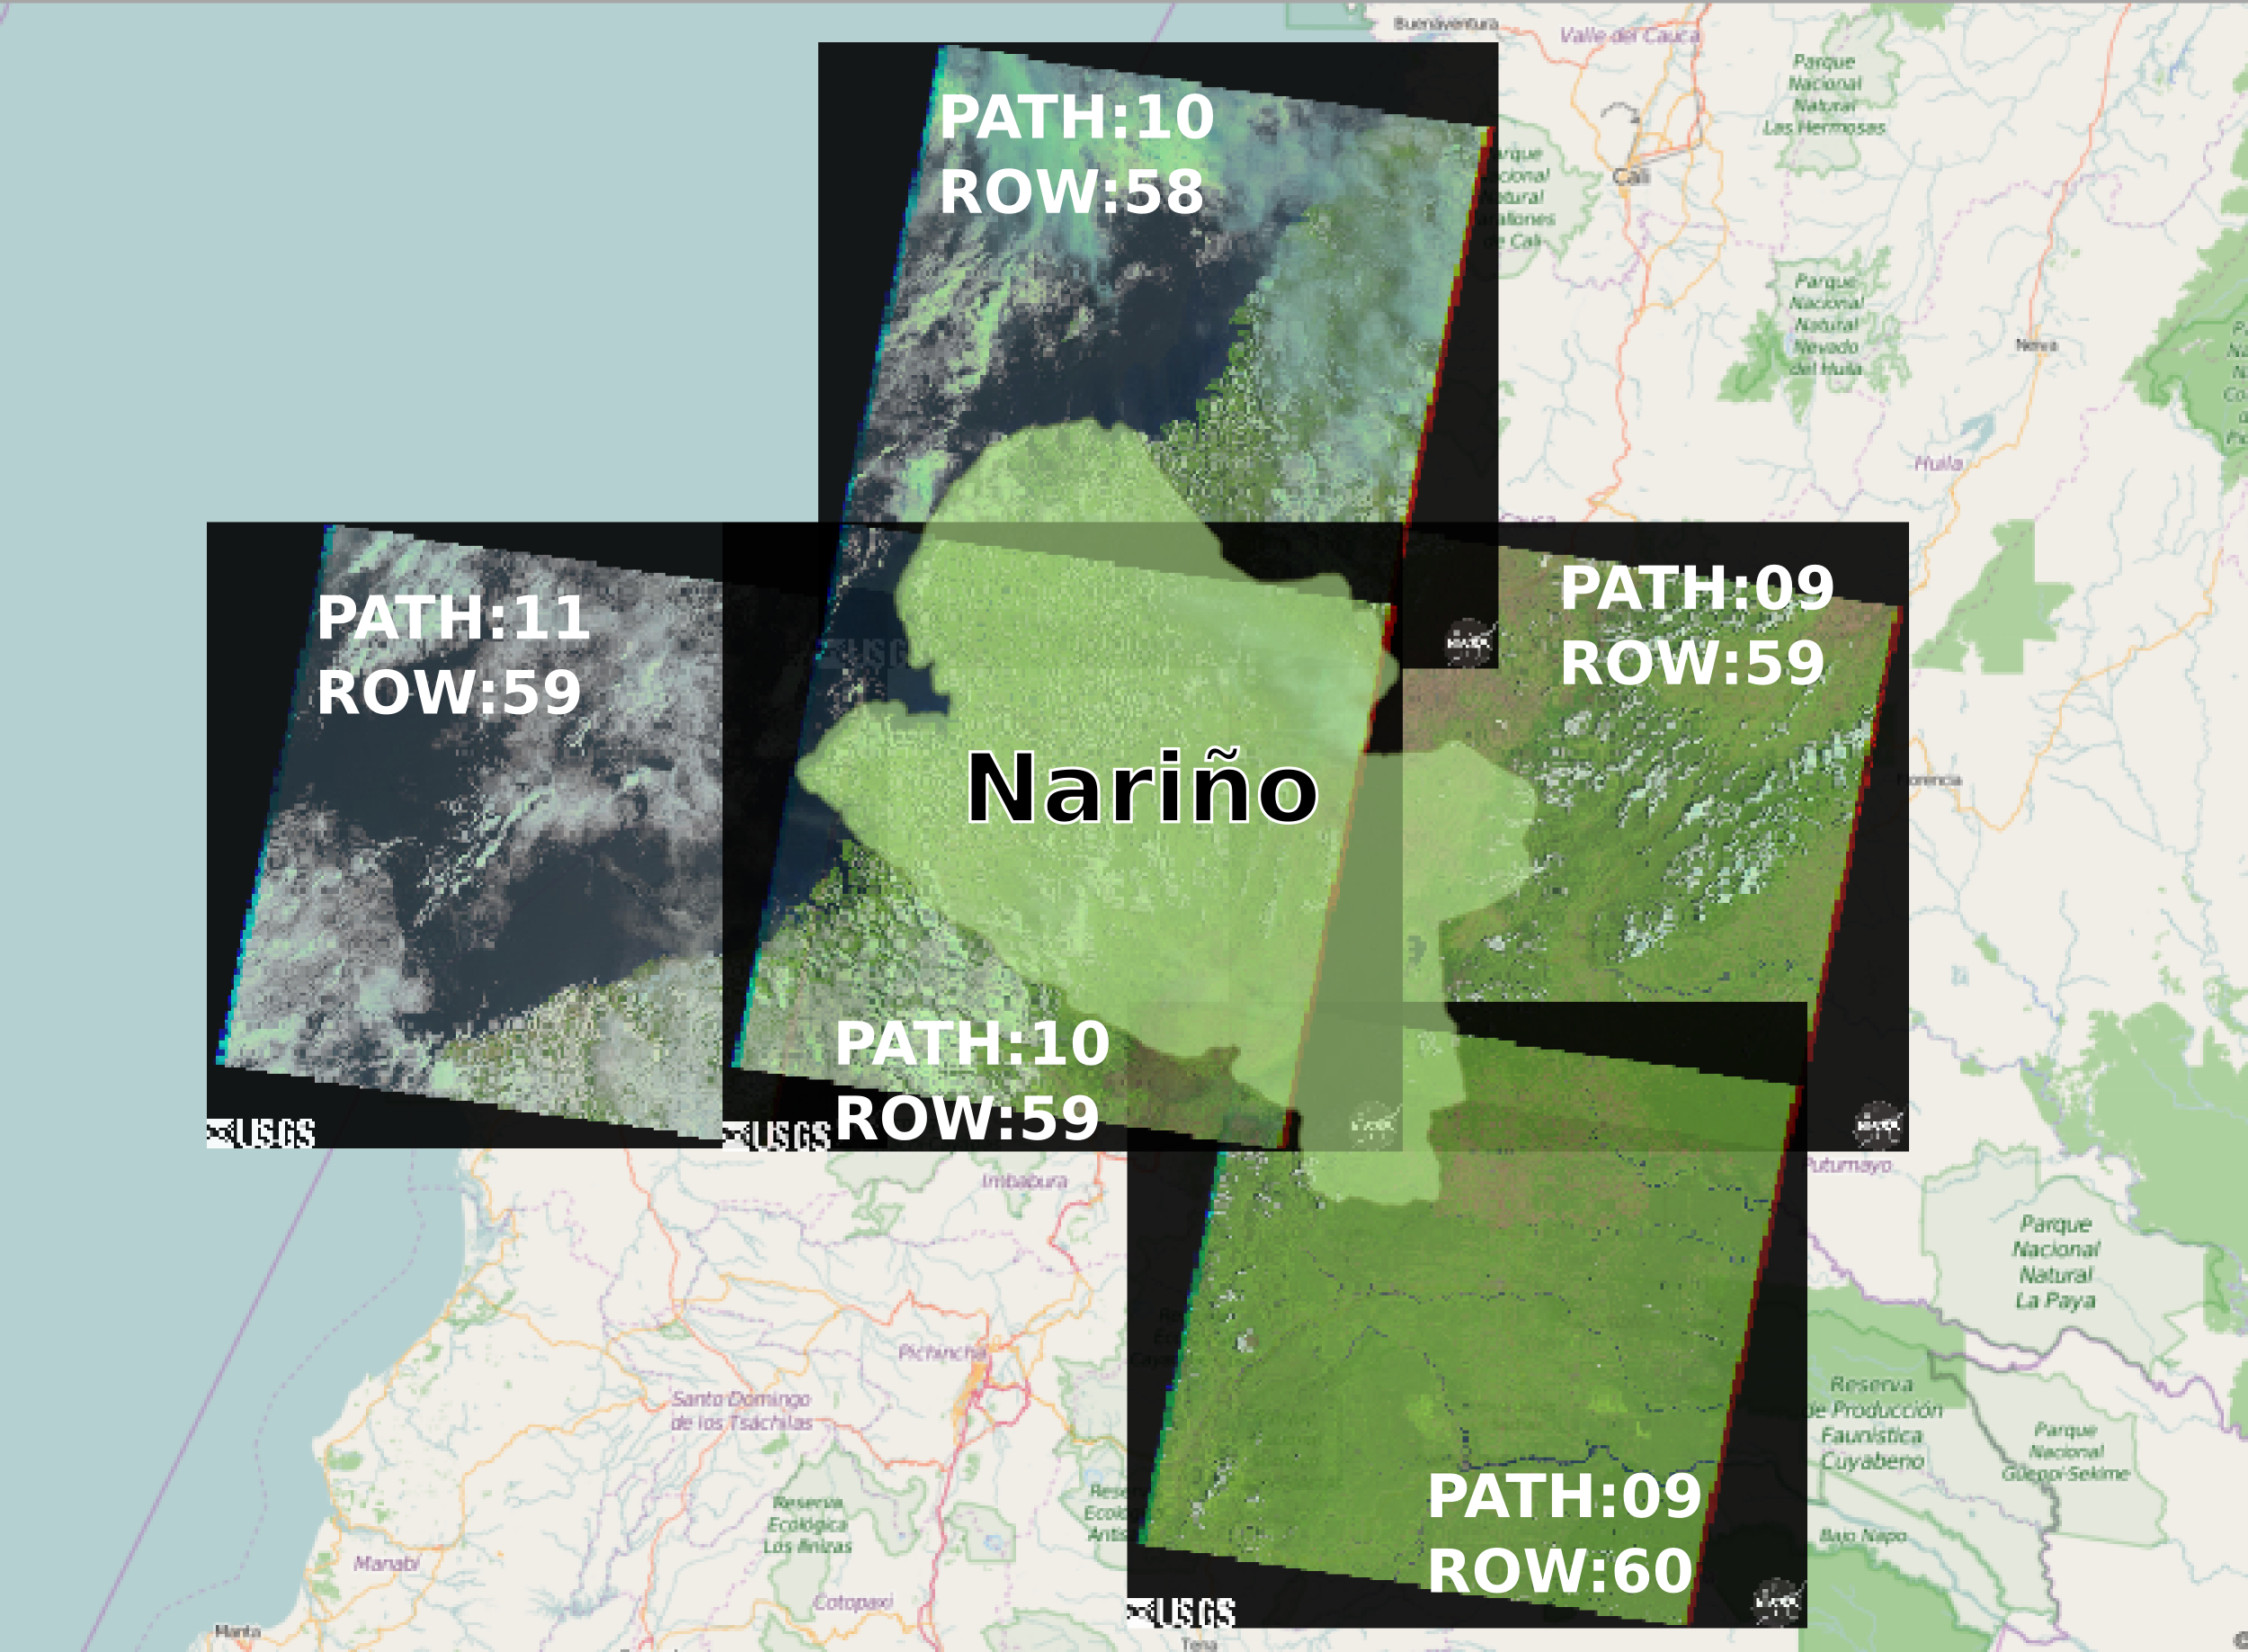
\includegraphics[width= 7cm]{cut1.png}}
  \vfill
  \subfigure[Imágenes recortadas de Nariño]{\label{Imágenes recortadas de Nariño}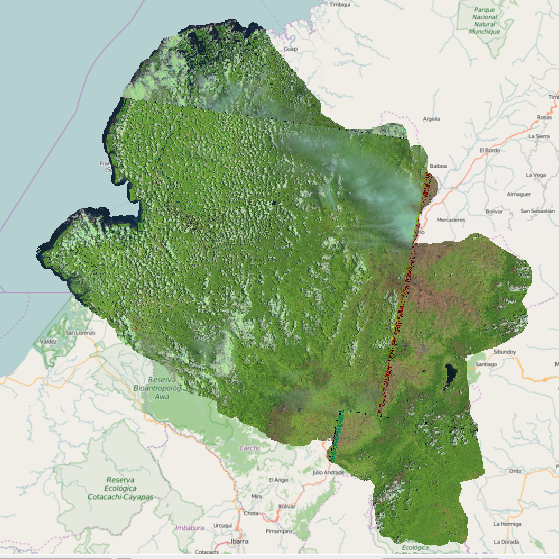
\includegraphics[width= 7cm]{cut2.png}}
  \caption{Prepocesamiento}
  \label{fig:Recortar imágenes}
\end{figure}

Para el caso de MODIS se convirtió el formato científico original de la imágen satelital(HDF) en un formato de imágenes
de mapa de bits (TIFF)
reproyectando el sistema de coordenadas espaciales original 
de  EPSG:4326 a EPSG:3857. Posterior a la conversión de formato y reproyección, 
se recortaron las imágenes satelitales con el fin unicamente de tener el área que cubre el departamento de Nariño.


\subsection{Procesamiento y limpieza de datos}

Se diseñaron dos base de datos, una para el sensor Landsat 7 y otra para el sensor MODIS.

El diseño de la base de datos para Landsat 7 lo muestra la figura~\ref{fig:landsatET}, la cual tiene 4 tablas. 

\begin{figure}
  \centering
  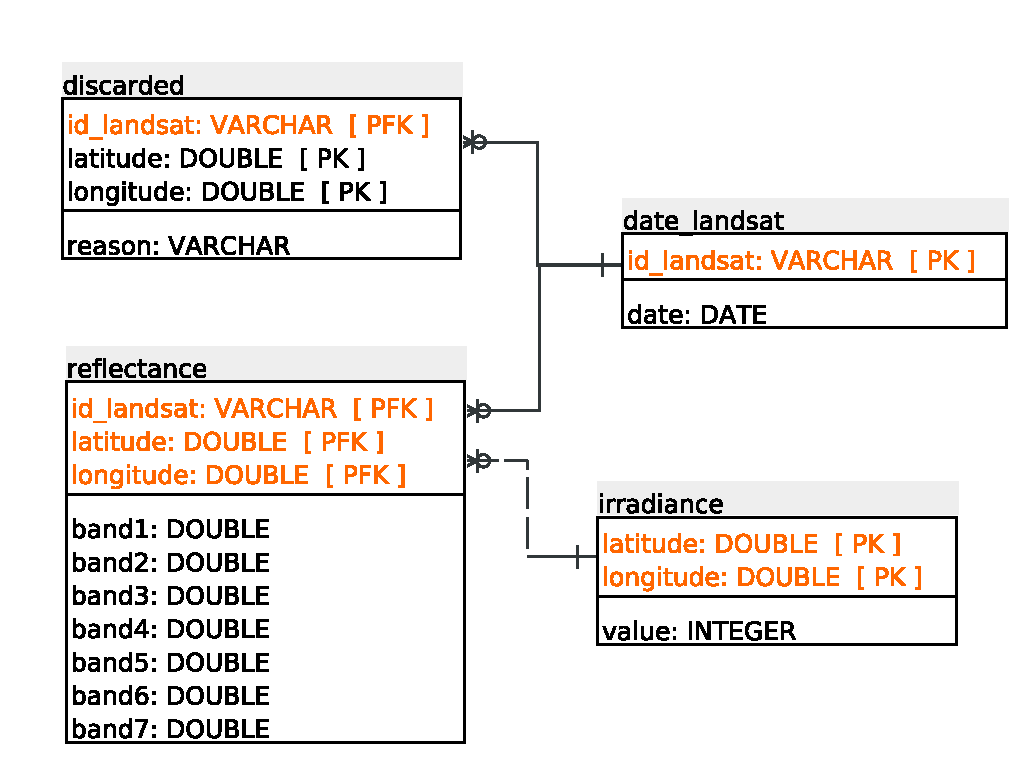
\includegraphics[width = 8cm]{landsatET.pdf}
  \caption{Modelo entidad-relacion Landsat}
  \label{fig:landsatET}
\end{figure}

Tabla date\_landsat: en la cual se almacenan las fechas de las imágenes satelitales.

Tabla reflectance: en la cual se almacenan los datos capturados y convertidos en reflentance,
de las bandas landsat (1 - 5,7) y la temperatura en grados kelvin de la banda 6.

Tabla discarded: en la cual se almacenan datos que fueron descartados, por varias razones,
son nubes calientes, nubes frias o ambiguos.

Tabla irradiance: en la cual se almacenan los datos de irradiance muestreados de 3TIER.

Para procesar las imágenes y llenar la base de datos se realizó un Script, el cual captura el Digital Number
de las imágenes satélitales y lo transforma en valor en reflectance. En este procesamiento de imagenes, se adiciono al Script unos filtros para para detección de nubes calientes,
nubes frias, datos ambiguos como lo muestra el algoritmo propuesto por \cite{irish2000landsat}. 

La tabla~\ref{tab:datos:landsat} muestra la relación de los datos obtenidos en este proceso.

\begin{table}
\caption{Datos obtenidos en en el proceso de procesamiento y limpieza  de datos Landsat 7}
\label{tab:datos:landsat}
\centering
\scalebox{0.7}{
\begin{tabular}{c c c}
\toprule
 Nombre & Valor& Detalle  \\
\midrule
Imágenes procesadas & 1321 & Imágenes de Nariño de 2000 a 2014 \\
Datos Totales & 51.076.512 & Registros Totales desde año 2000 a 2014 \\
Nube caliente & 3.731.768 & Registros de 2000 a 2014 \\
Nube Fria & 27.827.009 & Registros de 2000 a 2014 \\
Ambiguo & 11.987.340 & Registros de 2000 a 2014 \\
Datos Validos Reflectance & 4.071.185 & Registros de 2000 a 2014 \\
\bottomrule
\end{tabular}}
\end{table}

El diseño de la base de datos para MODIS lo muestra la figura~\ref{fig:modisET}, la cual tiene 4 tablas.

\begin{figure}
  \centering
  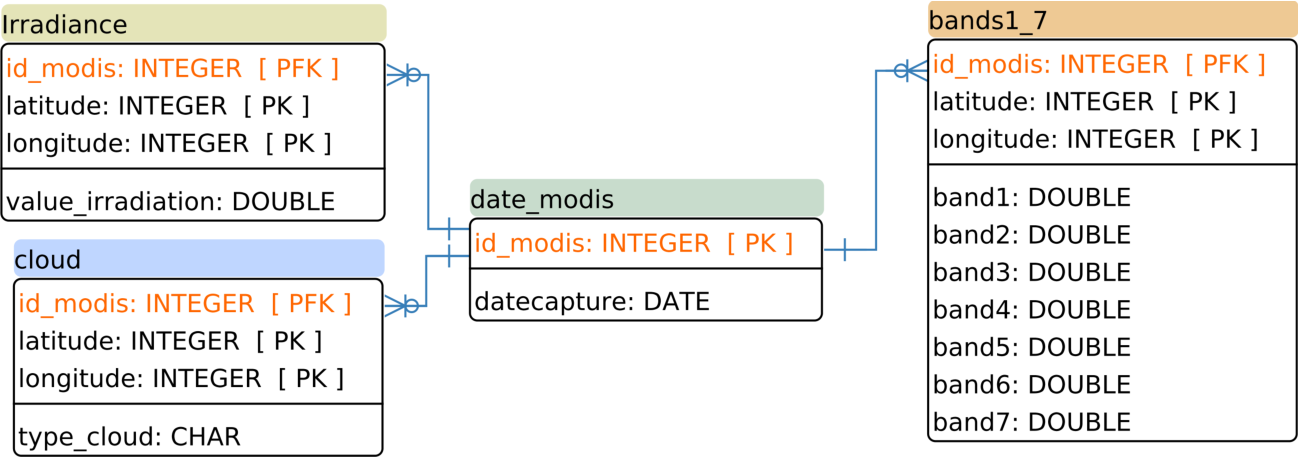
\includegraphics[width = 8cm]{bdmodis.pdf}
  \caption{Modelo entidad-relacion MODIS}
  \label{fig:modisET}
\end{figure}

Tabla date\_modis: en la cual se almacenan las fechas de las imágenes satelitales.

Tabla bands1\_7: se almacenan los valores de las bandas 1 a 7. 

Tabla cloud: se almacenan las coordenadas donde hay nubes.

Tabla irradiance: en la cual se almacenan los datos de irradiance muestreados de 3TIER.

Para procesar las imágenes y llenar la base de datos se realizó un Script, el cual recorre las 7 bandas en formato TIFF obtenidas del producto 
MOD09GA, se almacenan datos cada 450 metros y se aplíca el filtro de nubes según las especificaciones de las bandas \cite{bandMODISspecification}.

La tabla~\ref{tab:datos:modis} muestra la relación de los datos obtenidos en este proceso.

\begin{table}
\caption{Datos obtenidos en en el proceso de procesamiento y limpieza  de datos MODIS}
\label{tab:datos:modis}
\centering
\scalebox{0.7}{
\begin{tabular}{c c c}
\toprule
 Nombre & Valor& Detalle  \\
\midrule
Imágenes procesadas & 3912 & Imágenes de Nariño de 2005 a 2015 \\
Datos Totales & 565.722.468 & Registros Totales desde año 2005 a 2015 \\
Nubes & 192.051.992 & Registros de 2005 a 2015 \\
Nube tipo 1 & 160.318.600 & Registros de 2005 a 2015 \\
Nube tipo 2 & 31.733.392 & Registros de 2005 a 2015 \\
Datos Válidos & 373.670.476 & Registros de 2005 a 2015 \\
\bottomrule
\end{tabular}}
\end{table}

\subsection{Análisis de regresión}

El análisis de regresión se realizó tomando los valores agrupados de las bandas del sensor landsat 7 entre el año 2000 a 2014
y el valor de irradiancia solar que fue muestreada en 3TIER, para obtener el mejor modelo se evaluo 13 modelos y
6 métricas, de la misma manera este proceso se lo realizo para los datos del sensor MODIS entre el año 2005 a 2015.

Para encontrar el mejor modelo se utilizo la biblioteca de código abierto rminer presentada
por \cite{cortez2010data} para la herramienta R.

En la tabla~\ref{tab:metricas:landsat} se muestra las métricas de los modelos analizadas y el mejor modelo escogido
para los datos obtenidos del sensor landsat 7 y en la tabla~\ref{tab:metricas:modis} se muestran para el sensor MODIS.

\begin{table}
\caption{Métricas de modelos analizados con datos del sensor Landsat 7}
\label{tab:metricas:landsat}
\centering
\scalebox{0.7}{
\begin{tabular}{c c c c c c c}
\toprule
 & SAE& MAE & RAE & RMSE & COR & R2 \\
\midrule
ctree & 771.66185 & 5.32181 & 33.37397 & 8.89544 & 0.85991 & 0.73945 \\
rpart & 819.97501 & 5.65500 & 35.4634 & 9.23174 & 0.84774 & 0.71865 \\
kknn & 583.3615 & 4.02318 & 25.23008 & 6.19161 & 0.93584 & 0.87580 \\
mlp & 558.43603 & 3.85128 & 24.15206 & 5.49114 & 0.94968 & 0.90189 \\
mlpe & \textbf{461.93253} & \textbf{3.18574} & \textbf{19.97834} & \textbf{4.73616} & \textbf{0.96292} & \textbf{0.92721} \\
ksvm & 574.76656 & 3.96391 & 24.85835 & 5.71528 & 0.94664 & 0.89613 \\
randomForest & 663.70528 & 4.57728 & 28.70490 & 6.89480 & 0.92117 & 0.84856 \\
mr & 752.19550 & 5.18756 & 32.53206 & 6.75745 & 0.92222 & 0.85049 \\
mars & 680.67053 & 4.69428 & 29.43864 & 6.34212 & 0.93186 & 0.86837 \\
cubist & 538.20590 & 3.71176 & 23.27712 & 6.34056 & 0.93141 & 0.86752 \\
plsr & 748.89239 & 5.16478 & 32.38920 & 6.76538 & 0.92208 & 0.85023 \\
cppls & 748.89239 & 5.16478 & 32.38920 & 6.76538 & 0.92208 & 0.85023 \\
\bottomrule
\end{tabular}}
\end{table}

\begin{table}
\caption{Métricas de modelos analizados con datos de MODIS}
\label{tab:metricas:modis}
\centering
\scalebox{0.7}{
\begin{tabular}{c c c c c c c}
\toprule
 & SAE& MAE & RAE & RMSE & COR & R2 \\
\midrule
ctree & 1360.88975 & 9.13349 & 60.07076 & 13.06545 & 0.64264 & 0.41299 \\
rpart & 1373.21922 & 9.21624 & 60.61499 & 14.14182 & 0.60074 & 0.36089 \\
kknn & 920.48535 & 6.17775 & 40.63096 & 10.31934 & 0.79280 & 0.62854 \\
mlp & 485.60361 & 3.25908 & 21.43493 & 4.51435 & 0.96284 & 0.92705 \\
mlpe & \textbf{443.11836} & \textbf{2.97395} & \textbf{19.55960} & \textbf{3.97730} & \textbf{0.97157} & \textbf{0.94394} \\
ksvm & 823.63424 & 5.52775 & 36.35587 & 8.12712 & 0.87861 & 0.77195 \\
randomForest & 1159.07988 & 7.77906 & 51.16271 & 11.04659 & 0.75129 & 0.56444 \\
mr & 597.58282 & 4.01062 & 26.37778 & 5.36391 & 0.94694 & 0.89670 \\
mars & 618.82261 & 4.15317 & 27.31532 & 5.47634 & 0.94475 & 0.89255 \\
cubist & 597.29188 & 4.00867 & 26.36494 & 5.36508 & 0.94688 & 0.89658 \\
plsr & 597.29188 & 4.00867 & 26.36494 & 5.36508 & 0.94688 & 0.89658 \\
cppls & 597.29188 & 4.00867 & 26.36494 & 5.36508 & 0.94688 & 0.89658 \\
\bottomrule
\end{tabular}}
\end{table}

Según las métricas SAE, MAE, RAE, RMSE, COR y $R^2$ evaluadas en los 13 modelos, se 
encuentra que el modelo más óptimo para extrapolar 
los datos de irradiación es ``mlpe'' (multilayer perceptron ensemble) este modelo se aplica a todos
los datos obtenidos y se encuentra el valor de irradiancia.


\subsection{Construcción de mapas}

Para la construcción de mapas del potencial solar se utilizó el método Kriging que provee una solución al problema 
de la estimación basada en un modelo continuo de variación espacial estocástica, el objetivo de Kriging es el de estimar el valor de una 
variable aleatoria, Z, en uno o más puntos no muestreados o sobre grandes bloques. 

El método Kriging recibe como entrada datos de la muestra, y una malla dependiendo de la resolución que se quiera obtener, por ello los datos de muestra se
obtuvieron aplicando el modelo obtenido en el análisis de regresión a datos agrupados en cada punto por mes, año y uno
general entre el año 2000 a 2014 para el sensor landsat 7 y 2005 a 2015 para el sensor MODIS; y se 
 construyó una malla con puntos regulares espaciados cada 450 metros. 
 
 En las figuras~\ref{fig:solarMes:landsat}, \ref{fig:solarAnio:landsat} y \ref{fig:solarTotal:landsat}  se muestra los mapas 
 obtenidos por meses, años y general entre el año 2000 a 2014 respectivamente con datos del sensor landsat 7. 
 
\begin{figure}
  \centering
  \includegraphics[width = 8cm]{monthsLandsat.pdf}
  \caption{Mapas solar por meses datos landsat}
  \label{fig:solarMes:landsat}
\end{figure}

\begin{figure}
  \centering
  \includegraphics[width = 8cm]{yearsLandsat.pdf}
  \caption{Mapas solar por años datos landsat}
  \label{fig:solarAnio:landsat}
\end{figure}

\begin{figure}
  \centering
  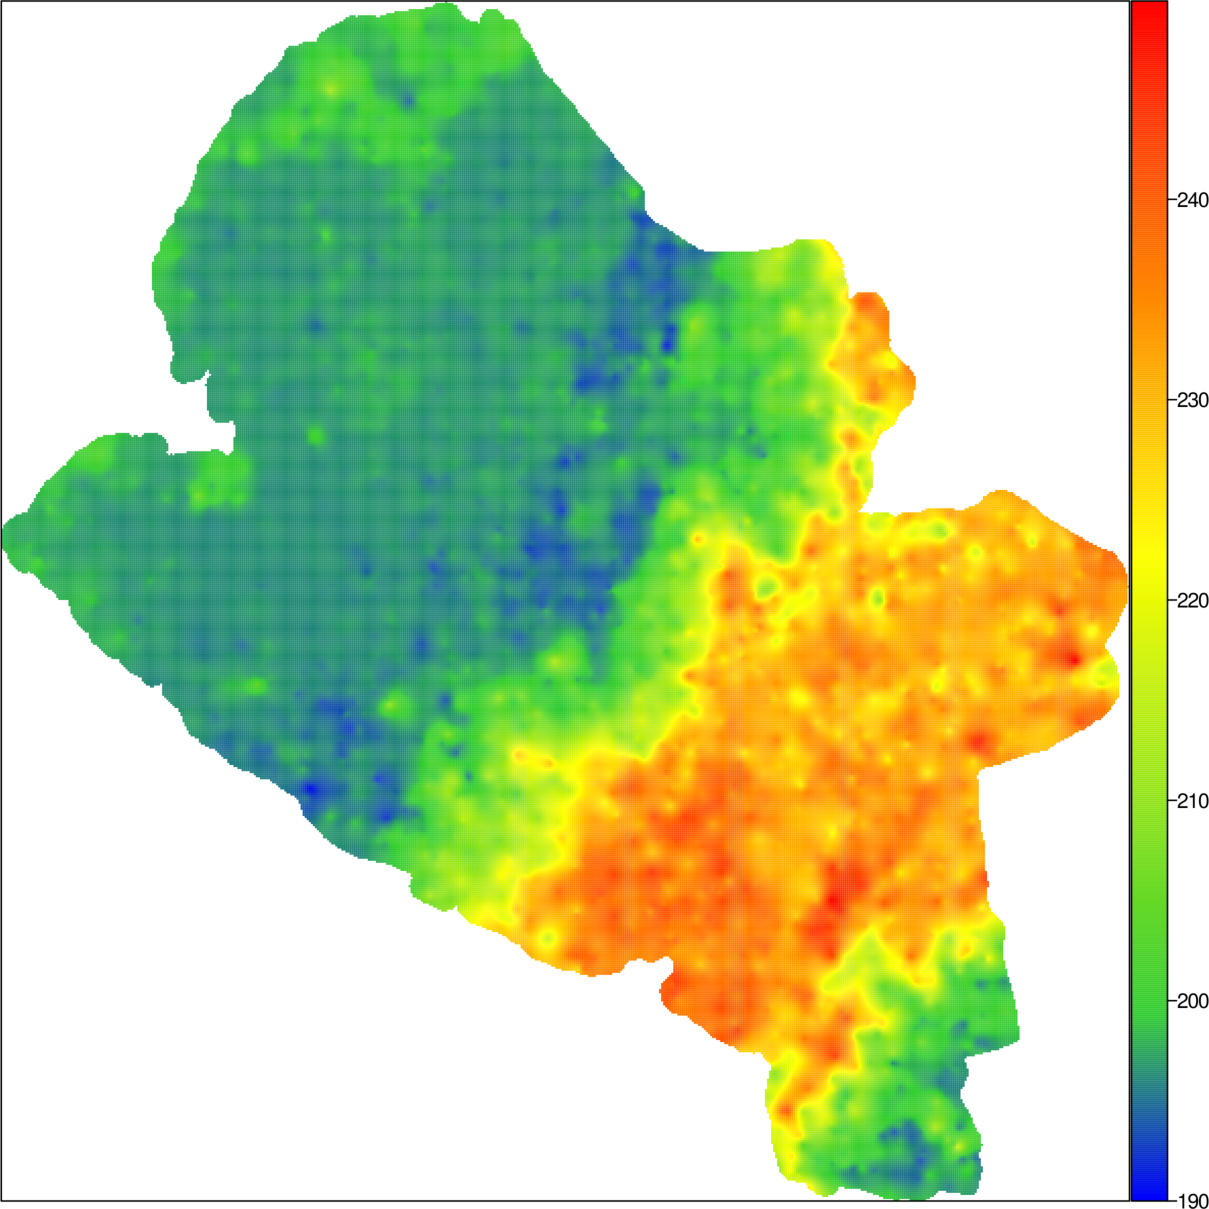
\includegraphics[width = 7cm]{generalLandsat.pdf}
  \caption{Mapas solar general años 2000-2014 datos landsat}
  \label{fig:solarTotal:landsat}
\end{figure}

 En las figuras~\ref{fig:solarMes:modis}, \ref{fig:solarAnio:modis} y \ref{fig:solarTotal:modis}  se muestra los mapas 
 obtenidos por meses, años y general entre el año 2005 a 2015 respectivamente con datos del sensor MODIS. 
 
\begin{figure}
  \centering
  \includegraphics[width = 8cm]{monthsModis.pdf}
  \caption{Mapas solar por meses datos MODIS}
  \label{fig:solarMes:modis}
\end{figure}

\begin{figure}
  \centering
  \includegraphics[width = 8cm]{yearsModis.pdf}
  \caption{Mapas solar por años datos MODIS}
  \label{fig:solarAnio:modis}
\end{figure}

\begin{figure}
  \centering
  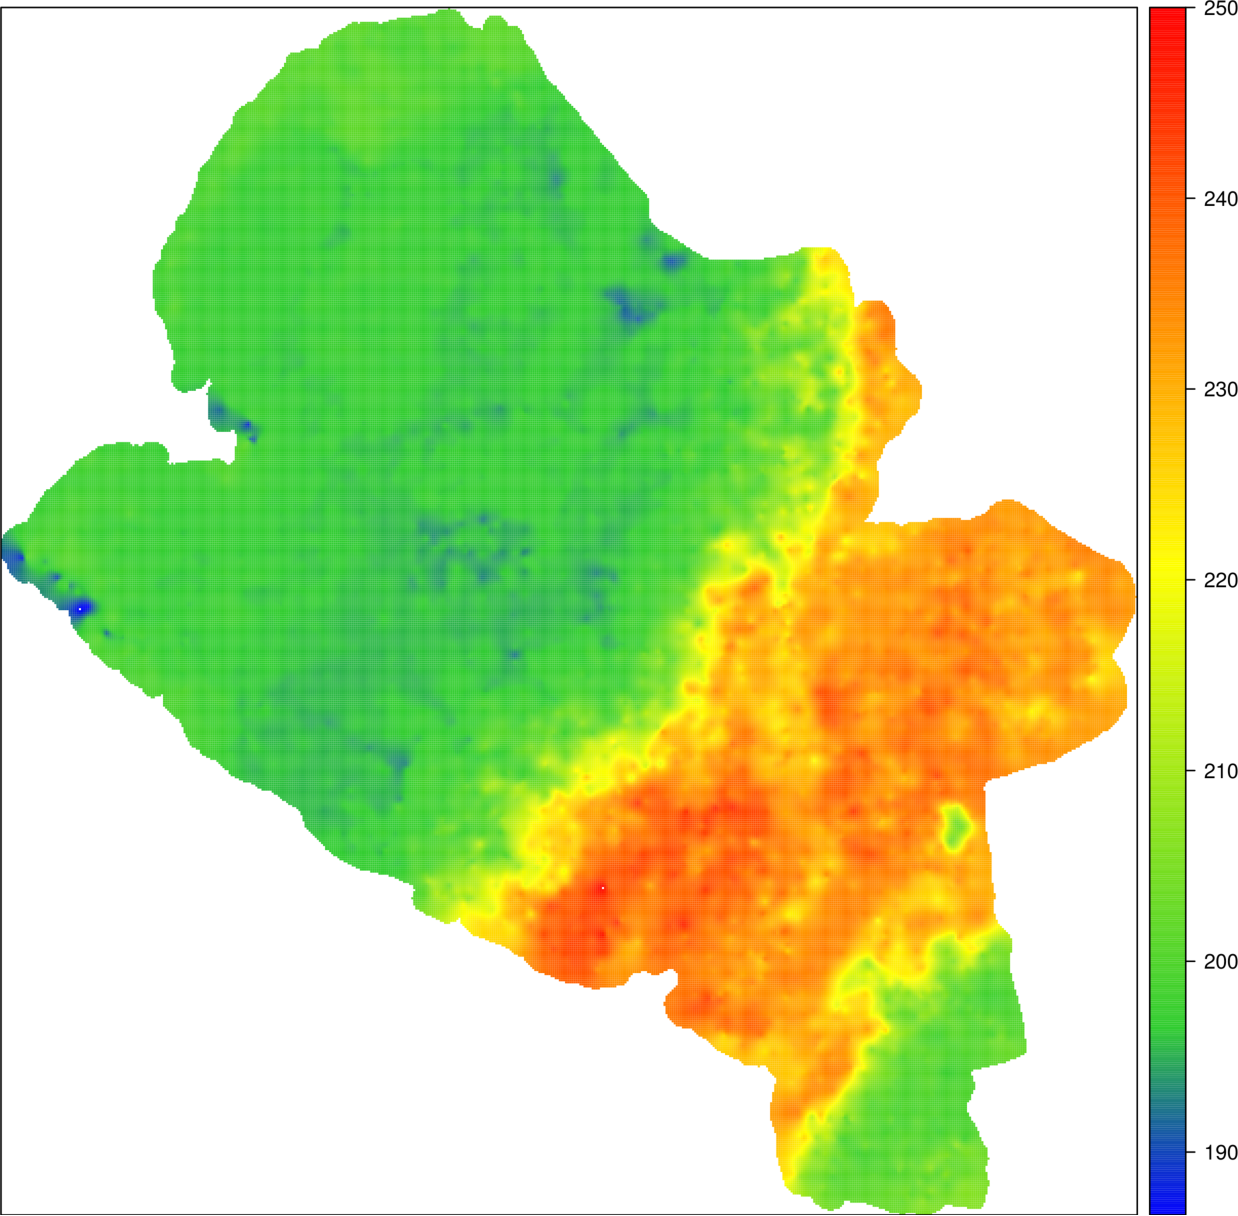
\includegraphics[width = 7cm]{generalModis.pdf}
  \caption{Mapas solar general años 2005-2015 datos MODIS}
  \label{fig:solarTotal:modis}
\end{figure}
